\begin{frame}{Algoritmos y técnicas utilizados}
	\begin{itemize}
		\item \textbf{Ingeniería de características Selección y creación de características}
			\begin{itemize}
				\item Selección de variables semánticamente representativas. 
				\item LasVegas Wrapper. 
				\item Imputación de valores perdidos con media o mediana.
				\item Creación de características. \pause 
			\end{itemize}
		\item \textbf{Técnicas basadas en instancias. Selección, eliminación de ruido, sobremuestreo}
			\begin{itemize}
				\item ENN.
				\item IPF.
				\item SMOTE. Oversampling
				\item Random Undersampling. \pause 
			\end{itemize}
		\item \textbf{Ajuste de hiperparámetros.}
			\begin{itemize}
				\item Gridsearch de parámetros F (número de folds), N (mínimo peso de instancias) y O (número de ejecución para optimizar).
				\item 5-CV.
			\end{itemize}
	\end{itemize}
\end{frame}
\subsection{Técnicas que no dan resultados}
\begin{frame}{Problemas con LasVegasWrapper}
	contenidos...
\end{frame}

\subsection{Técnicas que dan resultados}


\begin{frame}{Resultados}
\begin{itemize}
	\item 27 subidas. Mejor resultado: 0.7869.
	\item Mejor posición: 1752. Posición actual (17/02): 1834
\end{itemize}
	\begin{figure}
		\centering
		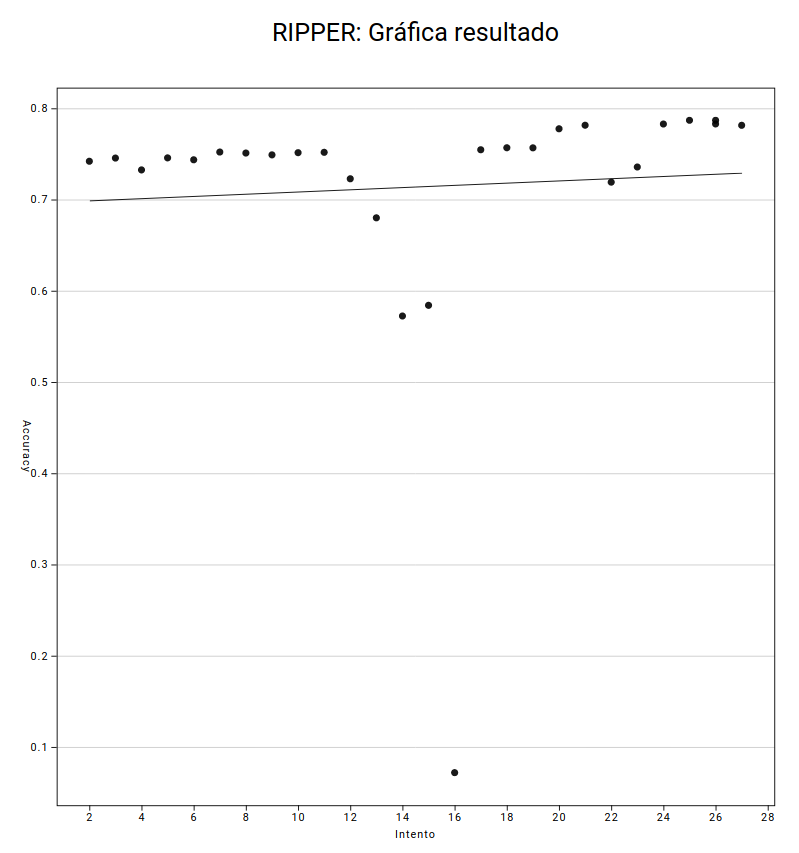
\includegraphics[scale=0.2]{figures/res-ripper.png}
		\caption{Gráfica de resultados}
	\end{figure}
\end{frame}

